\documentclass[10pt,a4paper,landscape]{article}
\usepackage[T1]{fontenc}
\usepackage[margin=1.6cm]{geometry}
\usepackage{underscore}
\usepackage{amsmath,amssymb}
\usepackage{booktabs,array,graphicx}
\usepackage{tikz}
\usetikzlibrary{arrows.meta,positioning,calc}
\setlength{\parindent}{0pt}
\setlength{\parskip}{4pt}
\pagestyle{empty}

\tikzset{
  >={Stealth[length=3mm,width=2.4mm]},
  box/.style={draw,rounded corners=2pt,align=center,fill=blue!6,font=\small,inner sep=4pt,minimum width=4.6cm,minimum height=1.5cm},
  file/.style={box,fill=green!10},
  hw/.style={box,fill=orange!15},
  tok/.style={draw,align=center,font=\small,minimum width=1.9cm,minimum height=0.8cm,fill=blue!6},
  data/.style={->,line width=0.9pt},
  lab/.style={font=\scriptsize,fill=white,inner sep=1pt,align=center}
}

\begin{document}

%==========================================================================
{\Large\bfseries 1. Language model: from sentences to the FPGA}

\medskip
\begin{center}
\resizebox{\textwidth}{!}{%
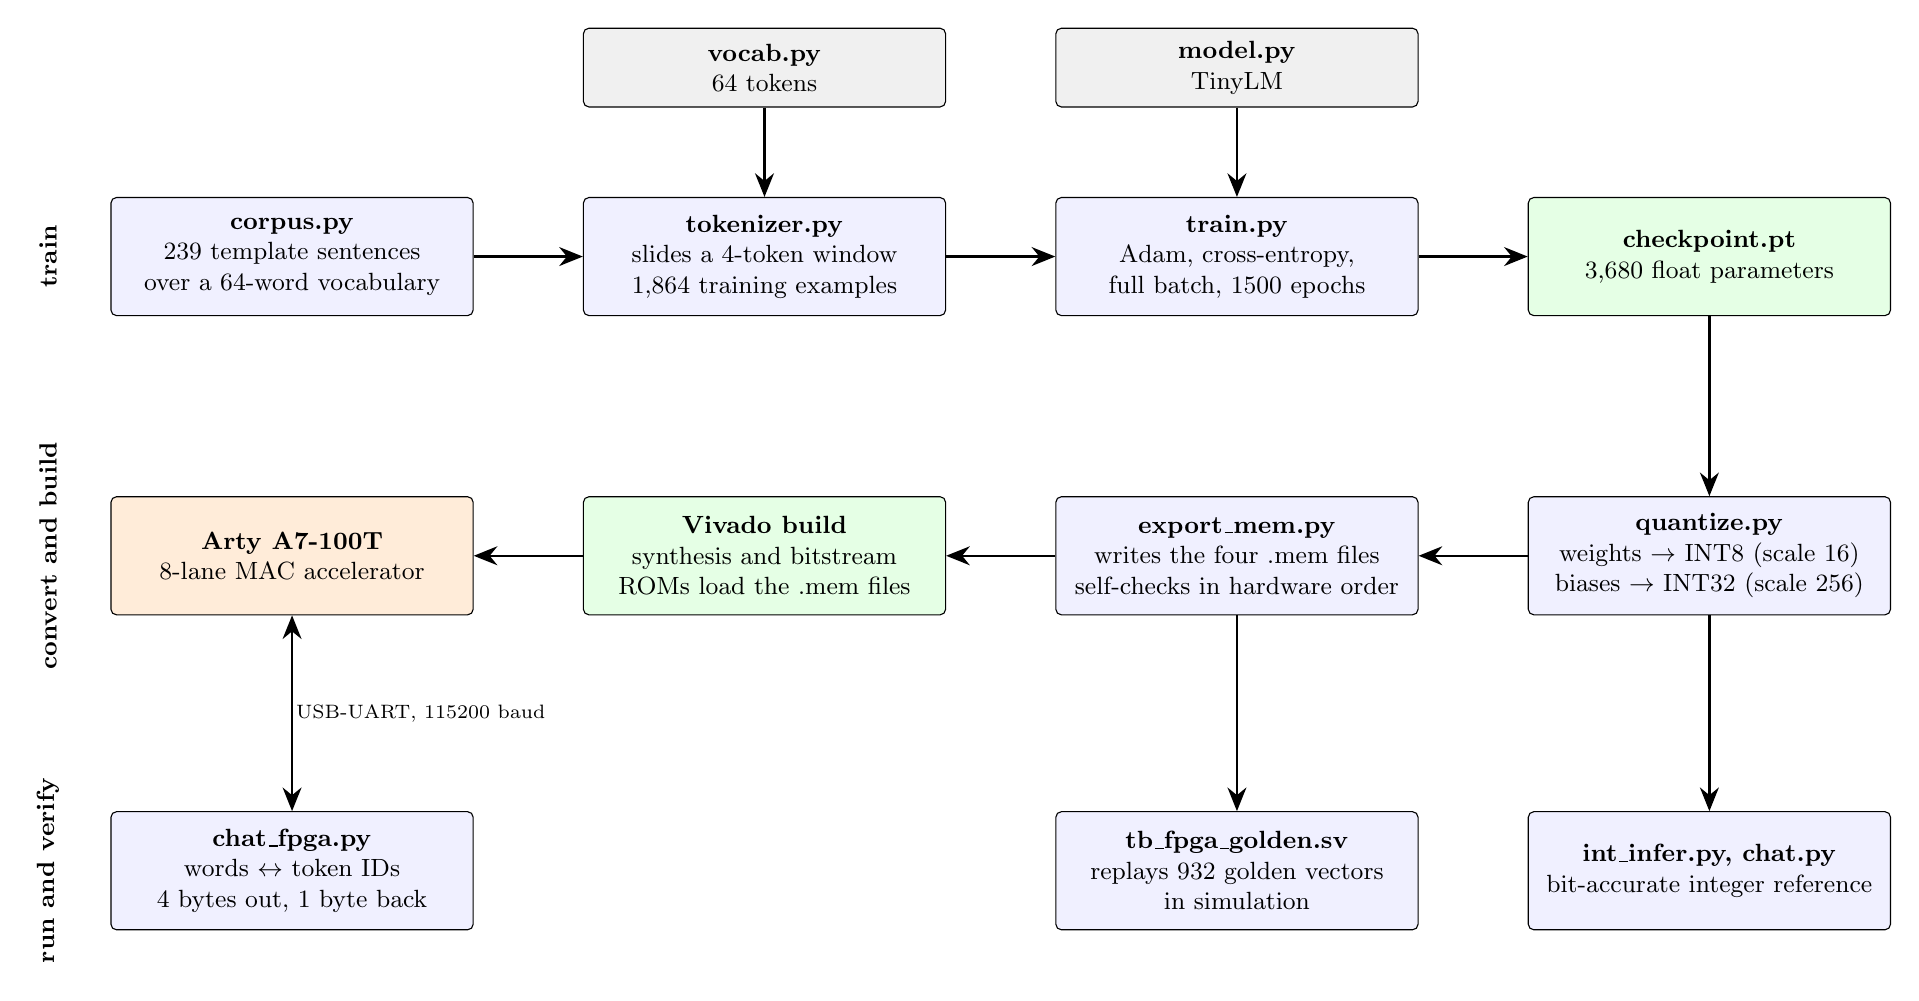
\begin{tikzpicture}
\node[box] (corpus)  at (0,7)    {\textbf{corpus.py}\\239 template sentences\\over a 64-word vocabulary};
\node[box] (tokenizer) at (6,7)  {\textbf{tokenizer.py}\\slides a 4-token window\\1,864 training examples};
\node[box] (train)   at (12,7)   {\textbf{train.py}\\Adam, cross-entropy,\\full batch, 1500 epochs};
\node[file] (ckpt)   at (18,7)   {\textbf{checkpoint.pt}\\3,680 float parameters};
\node[box,minimum height=1.0cm,fill=gray!12] (vocab) at (6,9.4)  {\textbf{vocab.py}\\64 tokens};
\node[box,minimum height=1.0cm,fill=gray!12] (model) at (12,9.4) {\textbf{model.py}\\TinyLM};
\draw[data] (corpus) -- (tokenizer);
\draw[data] (tokenizer) -- (train);
\draw[data] (train) -- (ckpt);
\draw[data] (vocab) -- (tokenizer);
\draw[data] (model) -- (train);

\node[box] (quant)   at (18,3.2) {\textbf{quantize.py}\\weights $\to$ INT8 (scale 16)\\biases $\to$ INT32 (scale 256)};
\node[box] (export)  at (12,3.2) {\textbf{export\_mem.py}\\writes the four .mem files\\self-checks in hardware order};
\node[file] (vivado) at (6,3.2)  {\textbf{Vivado build}\\synthesis and bitstream\\ROMs load the .mem files};
\node[hw]   (fpga)   at (0,3.2)  {\textbf{Arty A7-100T}\\8-lane MAC accelerator};
\draw[data] (ckpt) -- (quant);
\draw[data] (quant) -- (export);
\draw[data] (export) -- (vivado);
\draw[data] (vivado) -- (fpga);

\node[box] (fpgachat) at (0,-0.8)  {\textbf{chat\_fpga.py}\\words $\leftrightarrow$ token IDs\\4 bytes out, 1 byte back};
\node[box] (golden)   at (12,-0.8) {\textbf{tb\_fpga\_golden.sv}\\replays 932 golden vectors\\in simulation};
\node[box] (intinfer) at (18,-0.8) {\textbf{int\_infer.py, chat.py}\\bit-accurate integer reference};
\draw[<->,line width=0.9pt] (fpga) -- node[right,lab]{USB-UART, 115200 baud} (fpgachat);
\draw[data] (export) -- (golden);
\draw[data] (quant) -- (intinfer);

\node[font=\small\bfseries,rotate=90] at (-3.1,7)    {train};
\node[font=\small\bfseries,rotate=90] at (-3.1,3.2)  {convert and build};
\node[font=\small\bfseries,rotate=90] at (-3.1,-0.8) {run and verify};
\end{tikzpicture}}
\end{center}

The only file the hardware side depends on is \texttt{checkpoint.pt}. Everything after it is deterministic: quantizing, writing the memory files, and checking them against the integer reference. If the model is retrained, one command (\texttt{python -m langModel.export\_mem}) regenerates all four files and re-verifies them.

\clearpage
%==========================================================================
{\Large\bfseries 2. The model}

\medskip
\begin{center}
\resizebox{\textwidth}{!}{%
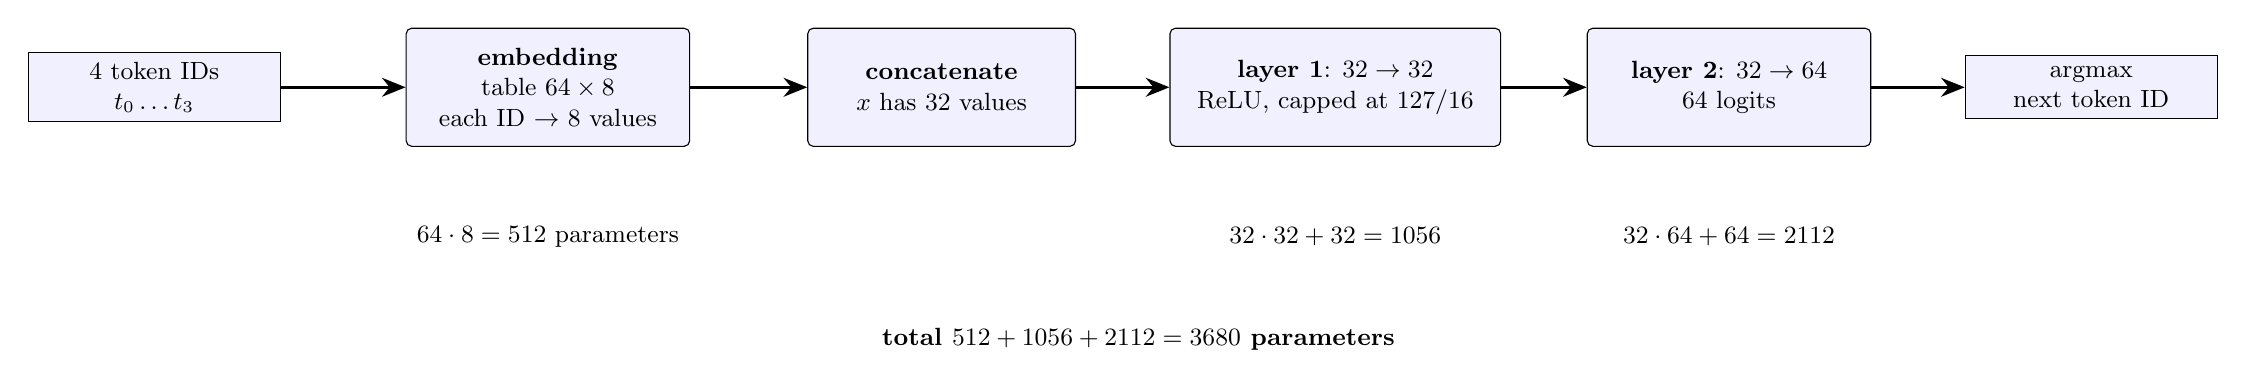
\begin{tikzpicture}
\node[tok,minimum width=3.2cm] (ids) at (0,0)  {4 token IDs\\{}$t_0\ldots t_3$};
\node[box,minimum width=3.6cm] (embed) at (5,0)  {\textbf{embedding}\\table $64\times 8$\\each ID $\to$ 8 values};
\node[box,minimum width=3.4cm] (cat) at (10,0)  {\textbf{concatenate}\\$x$ has 32 values};
\node[box,minimum width=4.2cm] (fc1) at (15,0)  {\textbf{layer 1}: $32\to 32$\\ReLU, capped at $127/16$};
\node[box,minimum width=3.6cm] (fc2) at (20,0)  {\textbf{layer 2}: $32\to 64$\\64 logits};
\node[tok,minimum width=3.2cm] (argmax) at (24.6,0) {argmax\\next token ID};
\foreach \a/\b in {ids/embed,embed/cat,cat/fc1,fc1/fc2,fc2/argmax}{\draw[data] (\a) -- (\b);}

\node[font=\small] at (5,-1.9)  {$64\cdot 8 = 512$ parameters};
\node[font=\small] at (15,-1.9) {$32\cdot 32 + 32 = 1056$};
\node[font=\small] at (20,-1.9) {$32\cdot 64 + 64 = 2112$};
\node[font=\small\bfseries] at (12.5,-3.2) {total $512 + 1056 + 2112 = 3680$ parameters};
\end{tikzpicture}}
\end{center}

\small
The cap on the hidden layer is the one thing that is not an ordinary ReLU. The hardware stores hidden activations as INT8 and clamps them to $[0,127]$ at scale 16, which is a real value of $127/16\approx 7.94$. Training uses the same cap (\texttt{HIDDEN\_MAX} in \texttt{model.py}), so the float model never relies on values the hardware cannot represent. It matters: about 10\% of hidden activations reach the cap.

\medskip
\begin{center}
\resizebox{0.95\textwidth}{!}{%
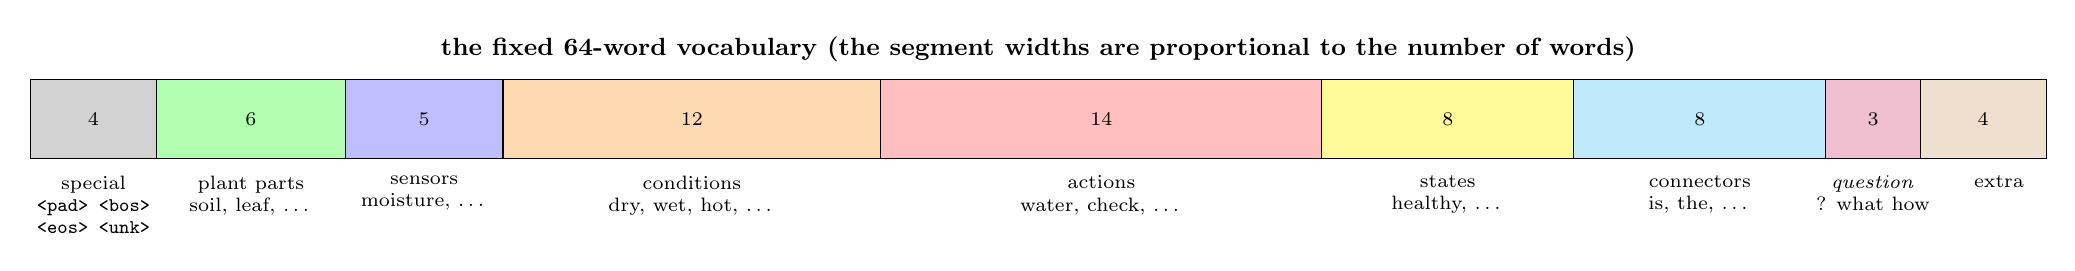
\begin{tikzpicture}
% vocabulary composition, one segment per group of the 64 tokens
\def\scale{0.125}
\fill[gray!35]   (0,0)       rectangle ({4*\scale*3.2},1);
\fill[green!30]  ({4*\scale*3.2},0)  rectangle ({10*\scale*3.2},1);
\fill[blue!25]   ({10*\scale*3.2},0) rectangle ({15*\scale*3.2},1);
\fill[orange!30] ({15*\scale*3.2},0) rectangle ({27*\scale*3.2},1);
\fill[red!25]    ({27*\scale*3.2},0) rectangle ({41*\scale*3.2},1);
\fill[yellow!40] ({41*\scale*3.2},0) rectangle ({49*\scale*3.2},1);
\fill[cyan!25]   ({49*\scale*3.2},0) rectangle ({57*\scale*3.2},1);
\fill[purple!25] ({57*\scale*3.2},0) rectangle ({60*\scale*3.2},1);
\fill[brown!25]  ({60*\scale*3.2},0) rectangle ({64*\scale*3.2},1);
\draw (0,0) rectangle ({64*\scale*3.2},1);
\foreach \x in {4,10,15,27,41,49,57,60}{\draw ({\x*\scale*3.2},0) -- ({\x*\scale*3.2},1);}
\node[font=\scriptsize,align=center] at ({2*\scale*3.2},0.5) {4};
\node[font=\scriptsize,align=center] at ({7*\scale*3.2},0.5) {6};
\node[font=\scriptsize,align=center] at ({12.5*\scale*3.2},0.5) {5};
\node[font=\scriptsize,align=center] at ({21*\scale*3.2},0.5) {12};
\node[font=\scriptsize,align=center] at ({34*\scale*3.2},0.5) {14};
\node[font=\scriptsize,align=center] at ({45*\scale*3.2},0.5) {8};
\node[font=\scriptsize,align=center] at ({53*\scale*3.2},0.5) {8};
\node[font=\scriptsize,align=center] at ({58.5*\scale*3.2},0.5) {3};
\node[font=\scriptsize,align=center] at ({62*\scale*3.2},0.5) {4};
\node[font=\scriptsize,anchor=north,align=center] at ({2*\scale*3.2},-0.1)    {special\\\texttt{<pad> <bos>}\\\texttt{<eos> <unk>}};
\node[font=\scriptsize,anchor=north,align=center] at ({7*\scale*3.2},-0.1)    {plant parts\\soil, leaf, \dots};
\node[font=\scriptsize,anchor=north,align=center] at ({12.5*\scale*3.2},-0.1) {sensors\\moisture, \dots};
\node[font=\scriptsize,anchor=north,align=center] at ({21*\scale*3.2},-0.1)   {conditions\\dry, wet, hot, \dots};
\node[font=\scriptsize,anchor=north,align=center] at ({34*\scale*3.2},-0.1)   {actions\\water, check, \dots};
\node[font=\scriptsize,anchor=north,align=center] at ({45*\scale*3.2},-0.1)   {states\\healthy, \dots};
\node[font=\scriptsize,anchor=north,align=center] at ({53*\scale*3.2},-0.1)   {connectors\\is, the, \dots};
\node[font=\scriptsize,anchor=north,align=center] at ({58.5*\scale*3.2},-0.1) {\textit{question}\\? what how};
\node[font=\scriptsize,anchor=north,align=center] at ({62.5*\scale*3.2},-0.1) {extra};
\node[font=\small\bfseries,anchor=south] at ({32*\scale*3.2},1.1) {the fixed 64-word vocabulary (the segment widths are proportional to the number of words)};
\end{tikzpicture}}
\end{center}

\clearpage
%==========================================================================
{\Large\bfseries 3. Training examples and the generation loop}

\medskip
\begin{center}
\resizebox{0.95\textwidth}{!}{%
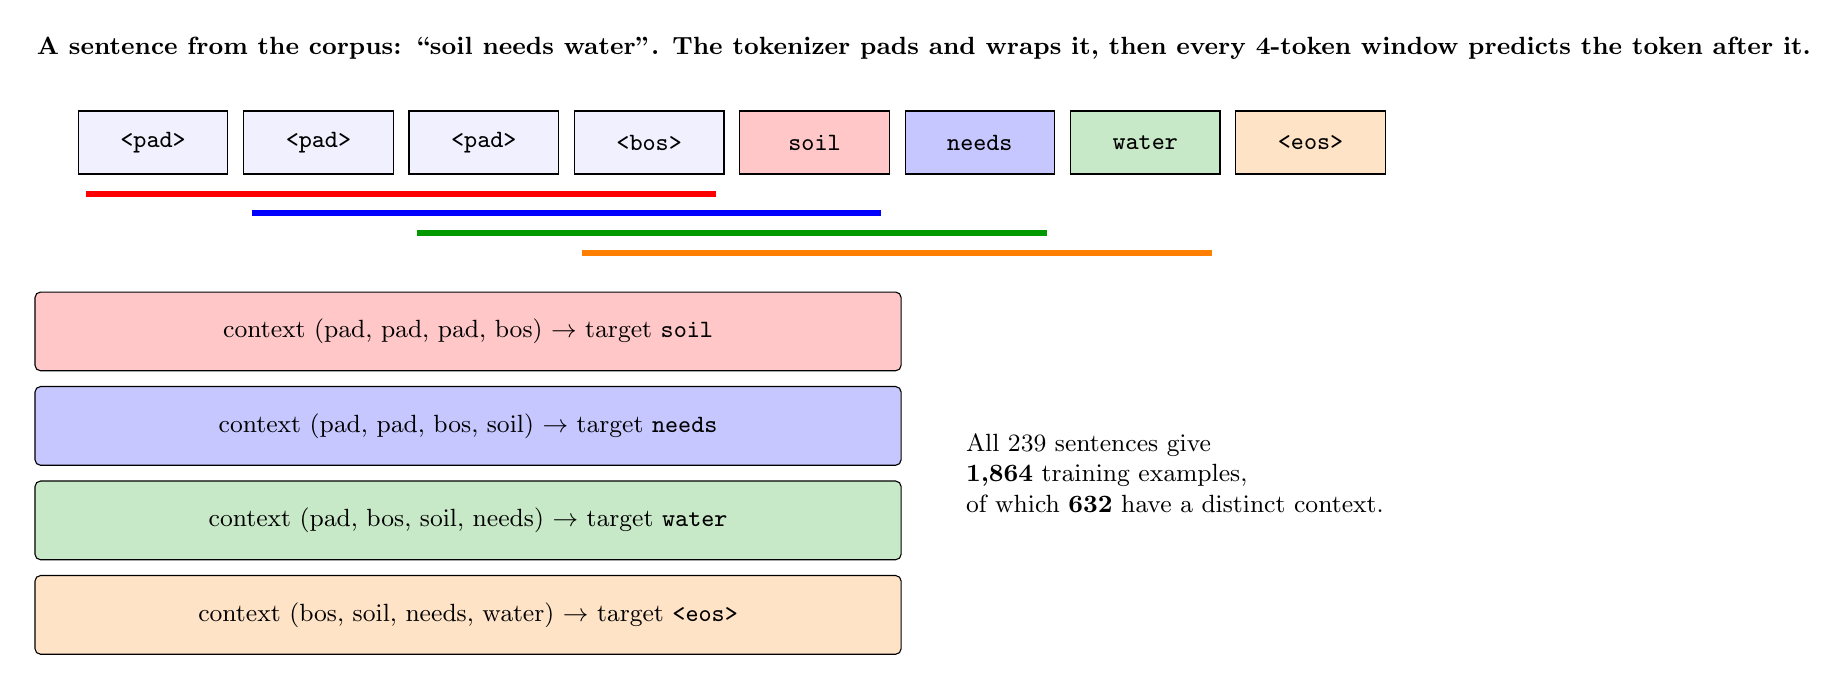
\begin{tikzpicture}
\node[font=\small\bfseries,anchor=west] at (-0.6,3.4) {A sentence from the corpus: ``soil needs water''. The tokenizer pads and wraps it, then every 4-token window predicts the token after it.};
\foreach \name/\i in {{<pad>}/0,{<pad>}/1,{<pad>}/2,{<bos>}/3}{
  \node[tok,fill=blue!6] at ({\i*2.1+1},2.2) {\texttt{\name}};
}
\foreach \name/\i/\col in {{soil}/4/red,{needs}/5/blue,{water}/6/green!60!black,{<eos>}/7/orange}{
  \node[tok,fill=\col!22] at ({\i*2.1+1},2.2) {\texttt{\name}};
}
\foreach \start/\col/\yy in {0/red/1.55,1/blue/1.3,2/green!60!black/1.05,3/orange/0.8}{
  \draw[line width=2.2pt,color=\col] ({\start*2.1+0.15},\yy) -- ({\start*2.1+8.15},\yy);
}
\node[box,fill=red!22,minimum width=11cm,minimum height=1.0cm,align=left,font=\small] at (5,-0.2) {context (pad, pad, pad, bos) $\to$ target \texttt{soil}};
\node[box,fill=blue!22,minimum width=11cm,minimum height=1.0cm,align=left,font=\small] at (5,-1.4) {context (pad, pad, bos, soil) $\to$ target \texttt{needs}};
\node[box,fill=green!60!black!22,minimum width=11cm,minimum height=1.0cm,align=left,font=\small] at (5,-2.6) {context (pad, bos, soil, needs) $\to$ target \texttt{water}};
\node[box,fill=orange!22,minimum width=11cm,minimum height=1.0cm,align=left,font=\small] at (5,-3.8) {context (bos, soil, needs, water) $\to$ target \texttt{<eos>}};
\node[font=\small,anchor=west,align=left] at (11.2,-2) {All 239 sentences give\\\textbf{1,864} training examples,\\of which \textbf{632} have a distinct context.};
\end{tikzpicture}}
\end{center}

\medskip
\begin{center}
\resizebox{\textwidth}{!}{%
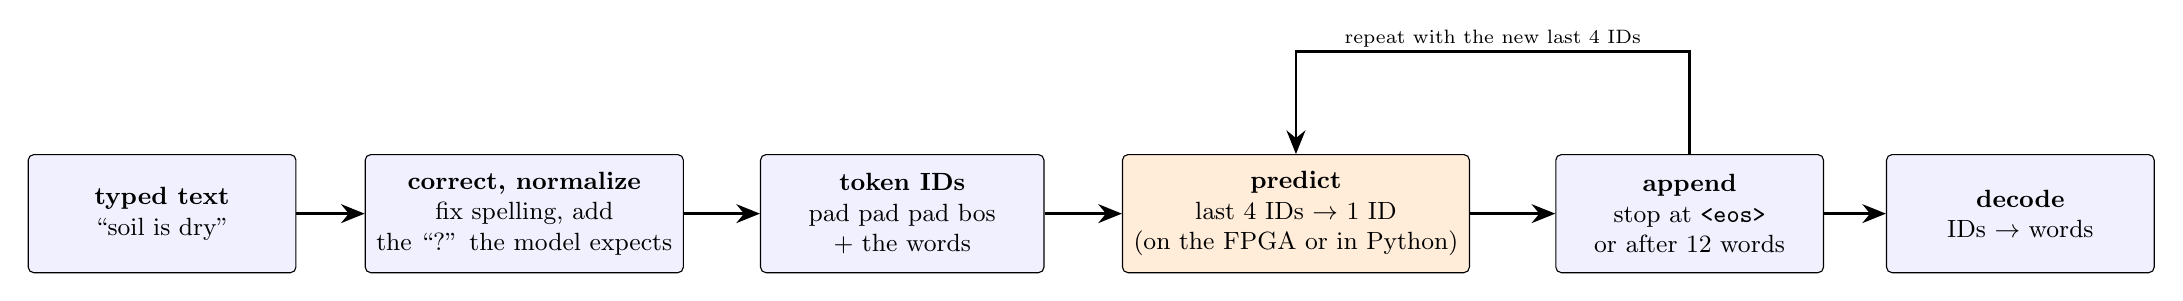
\begin{tikzpicture}
\node[box,minimum width=3.4cm] (text)   at (0,0)    {\textbf{typed text}\\``soil is dry''};
\node[box,minimum width=3.8cm] (clean)  at (4.6,0)  {\textbf{correct, normalize}\\fix spelling, add\\the ``?'' the model expects};
\node[box,minimum width=3.6cm] (ids)    at (9.4,0)  {\textbf{token IDs}\\pad pad pad bos\\+ the words};
\node[hw,minimum width=4.0cm]  (predict) at (14.4,0) {\textbf{predict}\\last 4 IDs $\to$ 1 ID\\(on the FPGA or in Python)};
\node[box,minimum width=3.4cm] (stop)   at (19.4,0) {\textbf{append}\\stop at \texttt{<eos>}\\or after 12 words};
\node[box,minimum width=3.4cm] (out)    at (23.6,0) {\textbf{decode}\\IDs $\to$ words};
\foreach \a/\b in {text/clean,clean/ids,ids/predict,predict/stop,stop/out}{\draw[data] (\a) -- (\b);}
\draw[data] (stop.north) -- ++(0,1.3) -| node[pos=0.25,above,lab]{repeat with the new last 4 IDs} (predict.north);
\end{tikzpicture}}
\end{center}

\small
The model only ever predicts one token. Autoregressive generation is the loop around it, which is why the hardware needs no tokenizer: the host sends 4 token IDs, receives 1, and does the rest.

\clearpage
%==========================================================================
{\Large\bfseries 4. Quantization and what the numbers look like}

\medskip
\begin{center}
\resizebox{0.9\textwidth}{!}{%
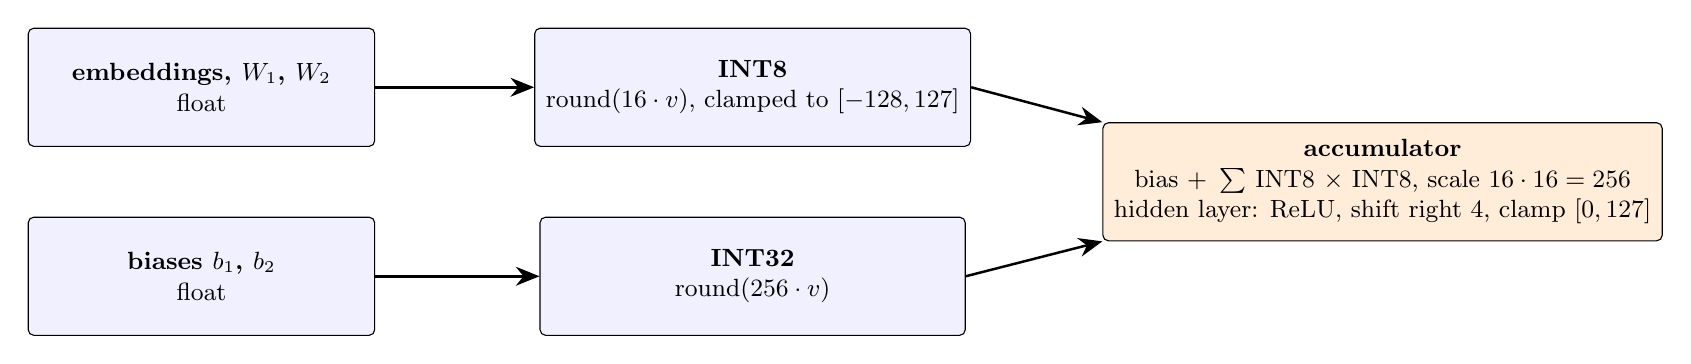
\begin{tikzpicture}
\node[box,minimum width=4.4cm] (f)  at (0,0)  {\textbf{embeddings, $W_1$, $W_2$}\\float};
\node[box,minimum width=5.4cm] (q8) at (7,0)  {\textbf{INT8}\\$\mathrm{round}(16\cdot v)$, clamped to $[-128,127]$};
\node[box,minimum width=4.4cm] (fb) at (0,-2.4) {\textbf{biases $b_1$, $b_2$}\\float};
\node[box,minimum width=5.4cm] (q32) at (7,-2.4) {\textbf{INT32}\\$\mathrm{round}(256\cdot v)$};
\node[box,minimum width=6.4cm,fill=orange!15] (acc) at (15,-1.2) {\textbf{accumulator}\\bias $+\ \sum$ INT8 $\times$ INT8, scale $16\cdot 16 = 256$\\hidden layer: ReLU, shift right 4, clamp $[0,127]$};
\draw[data] (f) -- (q8);
\draw[data] (fb) -- (q32);
\draw[data] (q8.east) -- (acc.north west);
\draw[data] (q32.east) -- (acc.south west);
\end{tikzpicture}}
\end{center}

\medskip
\begin{center}
\resizebox{\textwidth}{!}{%
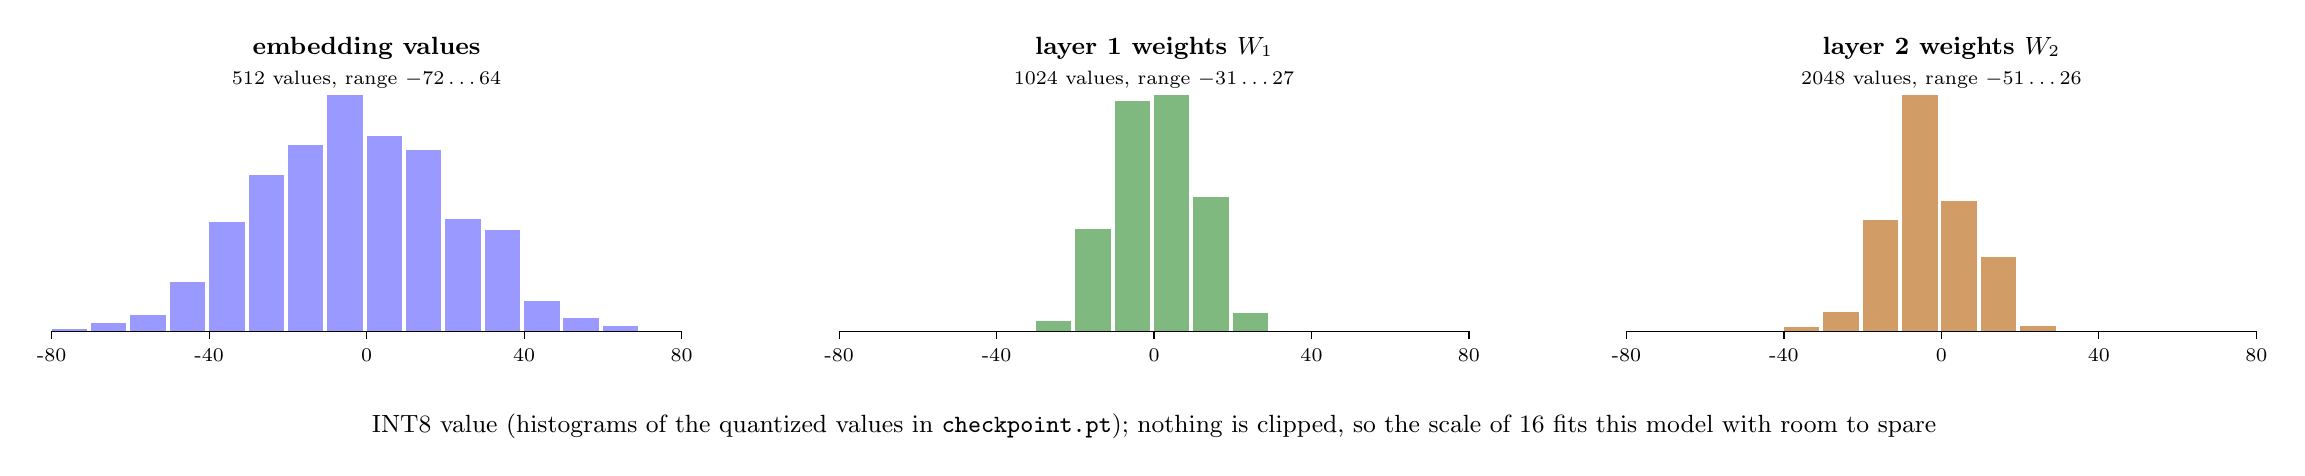
\begin{tikzpicture}
% three histograms of the INT8 values, bins of width 10 from -80 to 80
\def\w{0.5}
\begin{scope}[xshift=0cm]
  \foreach \cnt [count=\i from 0] in {1,3,6,18,40,57,68,86,71,66,41,37,11,5,2,0}{
    \fill[blue!40] ({\i*\w},0) rectangle ({\i*\w+\w*0.9},{\cnt*0.0349});}
  \draw (0,0) -- (8,0);
  \foreach \v/\p in {-80/0,-40/4,0/8,40/12,80/16}{\draw ({\p*\w},0) -- ({\p*\w},-0.1); \node[font=\scriptsize,anchor=north] at ({\p*\w},-0.1) {\v};}
  \node[font=\small\bfseries] at (4,3.6) {embedding values};
  \node[font=\scriptsize] at (4,3.2) {512 values, range $-72\ldots 64$};
\end{scope}
\begin{scope}[xshift=10cm]
  \foreach \cnt [count=\i from 0] in {0,0,0,0,1,14,143,322,330,188,26,0,0,0,0,0}{
    \fill[green!45!black!50] ({\i*\w},0) rectangle ({\i*\w+\w*0.9},{\cnt*0.00909});}
  \draw (0,0) -- (8,0);
  \foreach \v/\p in {-80/0,-40/4,0/8,40/12,80/16}{\draw ({\p*\w},0) -- ({\p*\w},-0.1); \node[font=\scriptsize,anchor=north] at ({\p*\w},-0.1) {\v};}
  \node[font=\small\bfseries] at (4,3.6) {layer 1 weights $W_1$};
  \node[font=\scriptsize] at (4,3.2) {1024 values, range $-31\ldots 27$};
\end{scope}
\begin{scope}[xshift=20cm]
  \foreach \cnt [count=\i from 0] in {0,0,1,1,17,69,392,830,458,261,19,0,0,0,0,0}{
    \fill[orange!70!black!60] ({\i*\w},0) rectangle ({\i*\w+\w*0.9},{\cnt*0.003614});}
  \draw (0,0) -- (8,0);
  \foreach \v/\p in {-80/0,-40/4,0/8,40/12,80/16}{\draw ({\p*\w},0) -- ({\p*\w},-0.1); \node[font=\scriptsize,anchor=north] at ({\p*\w},-0.1) {\v};}
  \node[font=\small\bfseries] at (4,3.6) {layer 2 weights $W_2$};
  \node[font=\scriptsize] at (4,3.2) {2048 values, range $-51\ldots 26$};
\end{scope}
\node[font=\small] at (14,-1.2) {INT8 value (histograms of the quantized values in \texttt{checkpoint.pt}); nothing is clipped, so the scale of 16 fits this model with room to spare};
\end{tikzpicture}}
\end{center}

\medskip
\footnotesize
\begin{center}
\begin{tabular}{@{}p{7.5cm}p{9.5cm}@{}}
\toprule
\textbf{Measured on \texttt{checkpoint.pt}} & \textbf{Result} \\
\midrule
Parameters, shapes & 3,680, all match the shared spec \\
INT8 values that clip & 0 of 3,584 \\
Largest accumulator magnitude over all 632 contexts & 20,262 (INT32 would overflow at 2,147,483,647) \\
Hidden activations: zero / between / at the cap 127 & 10,102 (50.0\%) / 8,139 (40.2\%) / 1,983 (9.8\%) \\
Accuracy on the training examples, float / integer & 75.3\% / 75.2\% \\
Float and integer argmax agree & 94.8\% of examples \\
\bottomrule
\end{tabular}
\end{center}
\small
The two models predict the same accuracy even though 5\% of individual argmax choices differ, so quantization is not what limits accuracy. Many contexts in the corpus legitimately have several valid next words, which caps what any model can score on them.

\clearpage
%==========================================================================
{\Large\bfseries 5. Files and how the export is checked}

\medskip
\small
\begin{center}
\begin{tabular}{@{}>{\ttfamily}p{3.6cm}p{13.4cm}@{}}
\toprule
\textbf{File} & \textbf{Role} \\
\midrule
vocab.py & the 64-word vocabulary and the ids of the special tokens \\
corpus.py & 239 sentences built from a few templates, including condition-to-advice tables \\
tokenizer.py & word $\leftrightarrow$ id, and the sliding 4-token window that makes (context, target) pairs \\
model.py & TinyLM: embedding, two linear layers, hidden activations capped at $127/16$ \\
train.py & full-batch Adam training, saves \texttt{checkpoint.pt}, prints sample generations \\
quantize.py & float $\to$ INT8 (scale 16) and INT32 (scale 256) \\
int\_infer.py & integer-only forward pass and generation loop: the reference the hardware must match exactly \\
export\_mem.py & reads the checkpoint (no PyTorch needed), writes the four \texttt{mem/} files, then verifies them \\
chat.py & text prompt loop on the integer reference (spelling correction, phrase normalizing) \\
chat\_fpga.py & the same loop with every prediction sent to the board over UART \\
\bottomrule
\end{tabular}
\end{center}

\medskip
\begin{center}
\resizebox{0.95\textwidth}{!}{%
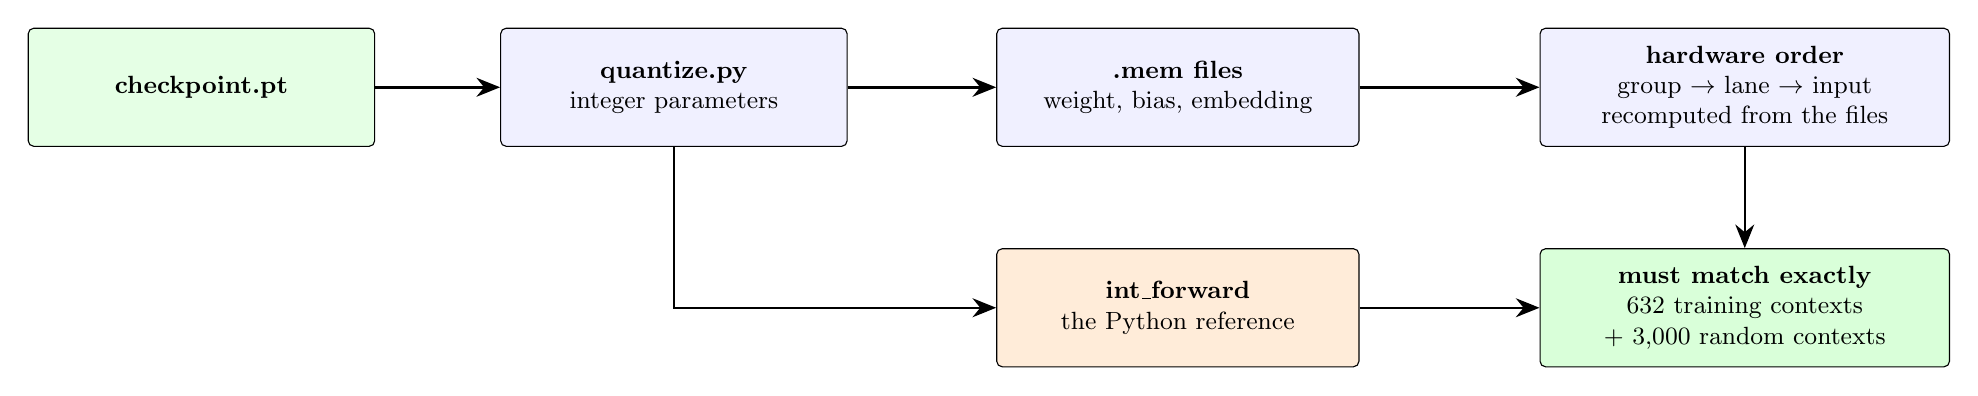
\begin{tikzpicture}
\node[file,minimum width=4.4cm] (ckpt) at (0,0) {\textbf{checkpoint.pt}};
\node[box,minimum width=4.4cm]  (ints) at (6,0) {\textbf{quantize.py}\\integer parameters};
\node[box,minimum width=4.6cm]  (mem)  at (12.4,0) {\textbf{.mem files}\\weight, bias, embedding};
\node[box,minimum width=5.2cm]  (hw)   at (19.6,0) {\textbf{hardware order}\\group $\to$ lane $\to$ input\\recomputed from the files};
\node[hw,minimum width=4.6cm]   (ref)  at (12.4,-2.8) {\textbf{int\_forward}\\the Python reference};
\node[box,minimum width=5.2cm,fill=green!15] (cmp) at (19.6,-2.8) {\textbf{must match exactly}\\632 training contexts\\+ 3,000 random contexts};
\draw[data] (ckpt) -- (ints);
\draw[data] (ints) -- (mem);
\draw[data] (mem) -- (hw);
\draw[data] (ints.south) |- (ref.west);
\draw[data] (ref) -- (cmp);
\draw[data] (hw) -- (cmp);
\end{tikzpicture}}
\end{center}

\small
This check runs every time the files are exported. It reads the written \texttt{.mem} files back, rebuilds the matrices exactly the way the hardware addresses them, and requires every one of the 64 logits to equal \texttt{int\_forward}'s. A mistake in the byte order or the address layout would fail here, before any Verilog is involved. The same export writes \texttt{golden\_vectors.mem}, which the simulation testbench replays through the real design.

\end{document}
